\chapter[As principais classes]{As principais classes: scrbook, scrreprt e scrartcl}
\begin{figure}[h]
    \centering
    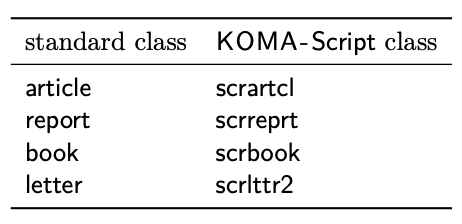
\includegraphics[width=0.60\linewidth]{classes.png}
    \caption{Principais Classes}
    \label{fig:class}
\end{figure}

Se você definir a opção dentro do documento, o tamanho da fonte principal e os tamanhos de fonte dependentes dos comandos \verb|\tiny|, \verb|\scriptsize|, \verb|\footnotesize|, \verb|\small|, \verb|\normalsize|, \verb|\large|, \verb|\Large|, \verb|\LARGE|, \verb|\huge| e \verb|\Huge| serão alterados. Isso pode ser útil, por exemplo, se você quiser que o apêndice seja definido em um tamanho de fonte menor.

Teoricamente, todas as declarações, incluindo texto literal, podem ser usadas como comandos. Você deve, no entanto, limitar-se àquelas declarações que realmente alteram apenas os atributos da fonte. Geralmente são comandos como \verb|\rmfamily|, \verb|\sffamily|, \verb|\ttfamily|, \verb|\upshape|, \verb|\itshape|, \verb|\slshape|, \verb|\scshape|, \verb|\mdseries|, \verb|\bfseries|, \verb|\normalfont|, bem como os comandos de tamanho de fonte \verb|\Huge|, \verb|\huge|, \verb|\LARGE|, \verb|\Large|, \verb|\large|, \verb|\normalsize|, \verb|\small|, \verb|\footnotesize|, \verb|\scriptsize| e \verb|\tiny|.

